\pdfoutput=1
\pdfminorversion=4
\pdfobjcompresslevel=0
% !TeX program = pdflatex
\documentclass[10pt,letterpaper]{article}

\usepackage{txbench-preprint}
\definecolor{todotext}{HTML}{A95F3D}
\newcommand{\todo}[1]{{\color{todotext}\textbf{[TODO:} #1\textbf{]}}}

\preprintKicker{bioRxiv preprint}
\preprintCategory{Computational Biology}
\preprintDate{June 2026}
\preprintTitle{TxBench-PP: Verifiable Evaluation of AI Agents on Preclinical Pharmacology}
\preprintAuthors{Hannah Le\preprintSup{1,*}, Ramesh Ramasamy\preprintSup{1,*}, Alex Urrutia\preprintSup{1,*}, Mahsa Yazdani\preprintSup{1,*}, Tim Proctor\preprintSup{1}, Kenny Workman\preprintSup{1}}
\preprintAffiliations{\preprintSup{1}LatchBio, San Francisco, CA, USA\\
\preprintSup{*}These authors contributed equally.}
\preprintCorrespondence{kenny@latch.bio}

\begin{document}

\PreprintHeader

\begin{PreprintAbstract}
We introduce TxBench-PP, a verifiable benchmark for evaluating AI agents on
small-molecule preclinical pharmacology. TxBench-PP is the first focused slice
of a broader TherapeuticsBench effort organized across drug-discovery stages
and therapeutic modalities. It targets recurring cluster-style decisions:
whether agents can recover decision-relevant conclusions from supplied assay
evidence rather than recalling drug labels, ranking by a single metric, or
applying generic checklists. The current task inventory is organized around
five evidence sources: decryptM dose-resolved phosphoproteomics, decryptE
expression proteomics, Kinobeads chemoproteomics target engagement,
TG-GATEs/DrugMatrix in vivo toxicogenomics, and a curated ADMET/DMPK/PK panel.
Together these datasets cover a small-molecule preclinical pharmacology spine:
mechanism of action and pharmacodynamics, compound-target engagement, ADMET
and PK, safety interpretation, and partial PK/PD translation. Agents receive
realistic workflow snapshots, inspect files in a coding environment, and return
structured answers graded deterministically. \todo{Replace this final
paragraph with model-run results: number of evaluations, model-harness pairs,
trajectories, top pass rates, and the main failure pattern.}
\end{PreprintAbstract}

\vfill
\clearpage

\section*{TxBench-PP in TherapeuticsBench}

{\fontsize{9.1}{12.8}\selectfont
TxBench-PP is the current small-molecule preclinical pharmacology slice of a
broader TherapeuticsBench roadmap. The full benchmark family is organized by
drug-discovery stage and therapeutic modality; this paper focuses on repeated,
verifiable cluster decisions in small-molecule programs. These decisions sit
between initial discovery and clinical development: whether a molecule engages
the intended biology, whether the evidence supports its mechanism, whether
exposure can cover the relevant potency range, and whether safety signals block
advancement.
\par}

\begin{center}
  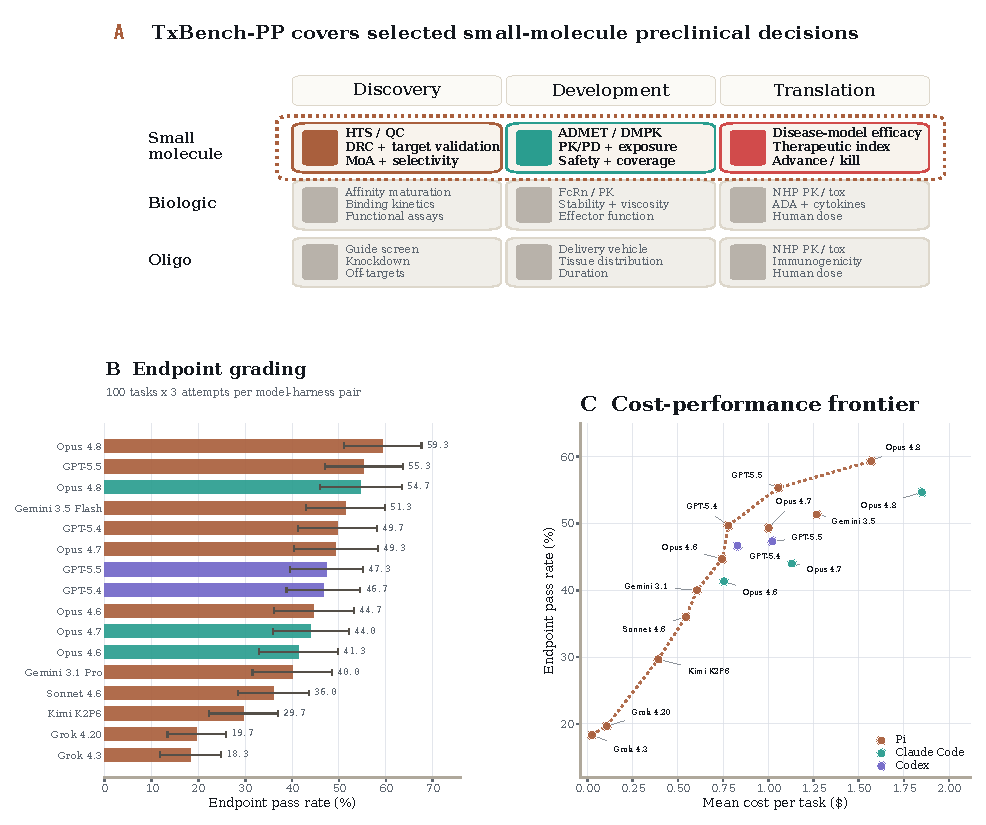
\includegraphics[width=0.96\textwidth]{figures/fig1_pipeline.pdf}

  \captionof{figure}{\textbf{TxBench-PP as a TherapeuticsBench slice.}
  TherapeuticsBench is intended to span discovery, development, and
  translation across small molecules, biologics, and oligonucleotides.
  TxBench-PP covers the small-molecule preclinical pharmacology slice as a
  cluster benchmark: repeated local decisions across assay families and
  compounds. Program-story benchmarks that follow one therapeutic program
  across discovery, development, and translation are reserved for future work.}
  \label{fig:pipeline-scope}
\end{center}

\clearpage

{\fontsize{9.1}{12.8}\selectfont
\newcommand{\TwoColParaBreak}{\par\vspace{0.62em}\noindent}
\noindent\begin{minipage}[t]{0.47\textwidth}
\setlength{\parskip}{0pt}
\setlength{\parindent}{0pt}

\section{Introduction}

In preclinical drug discovery, experiments are slow and expensive, but many
program-limiting decisions are interpretive: which signal is real, which
compound should advance, and which liability should block a program.
Preclinical pharmacology converts assay evidence into these decisions. A
compound can have an attractive potency value and still be a poor candidate
because the apparent mechanism is an artifact, the engaged protein is a complex
contaminant, the safety signal is protocol-specific, or total exposure does not
translate into unbound target coverage.

\TwoColParaBreak
AI agents can inspect files, write analysis scripts, and invoke scientific
software, but their conclusions often remain vulnerable to plausible shortcuts.
In drug discovery, those shortcuts have familiar forms: importing the known
mechanism of a blinded compound, trusting the largest apparent effect without
quality control, ranking by potency or total exposure alone, or applying a
textbook safety threshold outside the protocol where it was defined.

\TwoColParaBreak
We introduce TxBench-PP, a benchmark for small-molecule preclinical
pharmacology decisions. It should be read as a focused cluster benchmark within
the broader TherapeuticsBench roadmap rather than as a complete test of drug
discovery. Each evaluation supplies the agent with realistic analysis artifacts
from one stage of the preclinical pharmacology evidence chain and asks for a
structured, deterministically gradable conclusion. The benchmark tests whether
an agent can recover the result supported by the provided evidence, not whether
it can recall a drug class, run a default workflow, or optimize for a single
number.

\TwoColParaBreak
The current benchmark centers on five data sources: decryptM, decryptE,
Kinobeads, TG-GATEs/DrugMatrix, and curated PK/ADMET fixtures. These datasets
cover mechanism and pharmacodynamic readouts, compound-target engagement,
in vivo toxicology, source reconciliation, and exposure-aware prioritization.
\todo{Add final run summary once result aggregation is complete.}

\end{minipage}\hfill
\begin{minipage}[t]{0.47\textwidth}
\setlength{\parskip}{0pt}
\setlength{\parindent}{0pt}

\section{Benchmark Construction}

To construct TxBench-PP, we decompose preclinical pharmacology workflows into
short, gradeable scientific decisions. Examples include identifying a
pathway-coherent mechanism from dose-resolved phosphoproteomics, separating
true chemoproteomic target engagement from complex contaminants, reconciling
conflicting clearance measurements, and integrating blood chemistry, pathology,
and survival into an in vivo safety call.

\TwoColParaBreak
This makes TxBench-PP a cluster-style benchmark: the same kind of decision is
tested repeatedly across assay contexts, compounds, and evidence sources.
Future TherapeuticsBench story evaluations can test the complementary skill of
following one therapeutic program across discovery, development, and
translation. TxBench-PP instead asks whether agents can make the local
scientific decisions that those longer program stories depend on.

\TwoColParaBreak
Each task includes a snapshot of assay outputs immediately before a target
decision, metadata needed to interpret the files, a high-level task
description, and a deterministic grader. Tasks specify what result should be
recovered rather than prescribing the exact analysis method. Procedural details
are included only when they are part of the scientific decision, such as
whether free or total exposure should be compared to a pharmacologic threshold.

\TwoColParaBreak
The benchmark follows three design criteria. First, tasks must be verifiable:
answers are checked by structured label matching, numerical tolerances,
rank-order checks, or all-of field comparisons. Second, tasks should be
decision-relevant: the answer should correspond to a real go/no-go or
prioritization judgment in preclinical pharmacology. Third, tasks should resist
shortcuts: agents should need to inspect the supplied evidence, account for
quality issues, and avoid relying on memorized drug labels or generic
checklists.

\TwoColParaBreak
We separately track decision-blocking gaps: issues that should change the
program decision if recognized, such as a tox-species mismatch, insufficient
free-drug coverage, a hook effect, a contaminated chemoproteomic hit, or
survivor bias in pathology sampling. These labels are intended to support
diagnostic analysis after endpoint grading.

\end{minipage}
}

\clearpage

{\fontsize{9.1}{12.8}\selectfont
\section{Evaluation Inventory}

\begin{multicols}{2}
The current suite is organized by assay evidence rather than by a generic drug
discovery checklist. decryptM and decryptE map to discovery-stage mechanism,
pathway, and pharmacodynamic reasoning from dose-resolved proteomic readouts.
Kinobeads sits at the discovery/development bridge by testing direct
target-engagement reasoning, including contaminant rejection and cluster-boundary
selection. PK/ADMET tasks map to development-stage exposure, clearance,
protein-binding, permeability, and source-reconciliation decisions. TG-GATEs
and DrugMatrix map to translation-facing safety interpretation across chemistry,
pathology, survival, and protocol context.
\par

The inventory intentionally leaves major parts of TherapeuticsBench outside the
current scope. Target genetics, disease-model characterization, broad
pharmacogenomics, primary screening QC, biologics developability, antibody-drug
conjugates, degraders, oligonucleotides, and cell or gene therapies are natural
future extensions, but are not required to define the small-molecule
preclinical pharmacology slice tested here.
\par
\end{multicols}
}

\begin{center}
  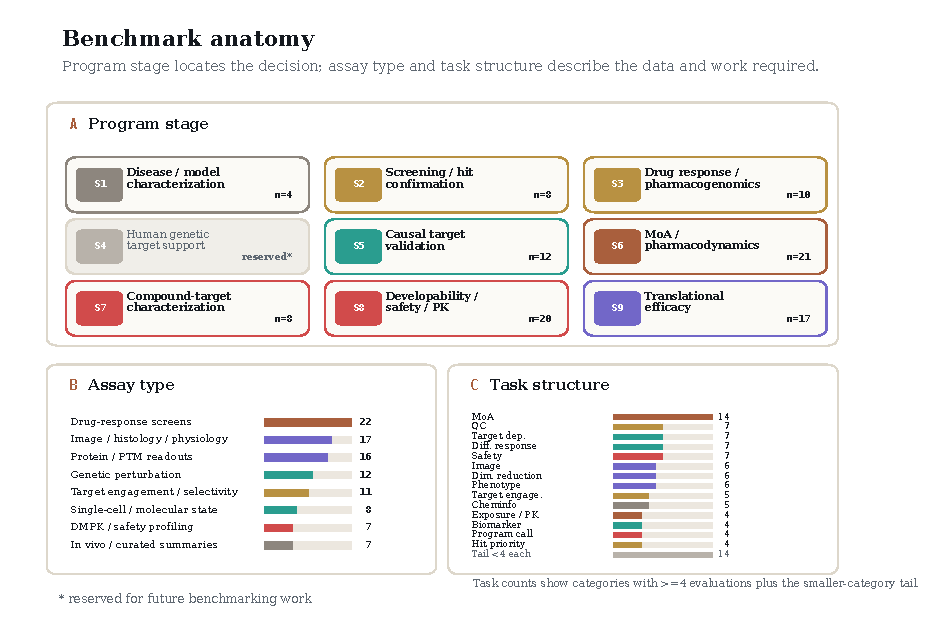
\includegraphics[width=0.94\textwidth]{figures/fig2_inventory.pdf}

  \captionof{figure}{\textbf{Evaluation inventory by evidence source.}
  Current TxBench-PP tasks are drawn from five small-molecule preclinical
  pharmacology evidence sources. Approximate evaluation counts come from the
  planning documents and should be replaced with frozen counts before
  submission.}
  \label{fig:evaluation-inventory}
\end{center}

\begin{center}
\fontsize{7.0}{8.5}\selectfont
\setlength{\tabcolsep}{3.2pt}
\begin{tabular}{@{}>{\raggedright\arraybackslash}p{0.13\linewidth}
                >{\centering\arraybackslash}p{0.055\linewidth}
                >{\raggedright\arraybackslash}p{0.25\linewidth}
                >{\raggedright\arraybackslash}p{0.43\linewidth}@{}}
\toprule
Evidence source & Evals & Assay evidence & Decision themes \\
\midrule
decryptM & 48 & dose-resolved phosphoproteomics &
Mechanism-of-action inference, pathway-coherent signalling, artifact rejection \\
\addlinespace
decryptE & 12 & dose-resolved expression proteomics &
Expression-proteomic pathway response, reliable target signal selection, single-feature artifact avoidance \\
\addlinespace
Kinobeads & 2 & chemoproteomics target engagement &
Direct target selection, contaminant removal, engaged-cluster boundary detection \\
\addlinespace
TG-GATEs / DrugMatrix & $\sim$20 & in vivo rat toxicogenomics and safety &
Integrated toxicity calls, pathology and chemistry reconciliation, survivor bias, species-specific artifacts \\
\addlinespace
PK / ADMET panel & $\sim$45 & ADMET, DMPK, PK, literature measurements &
Clearance source reconciliation, free-drug exposure, safety margins, potency-adjusted prioritization \\
\bottomrule
\end{tabular}
\captionof{table}{\textbf{Draft TxBench-PP inventory.}
The current benchmark should be described as a small-molecule preclinical
pharmacology suite. Counts marked with $\sim$ should be replaced when the final
evaluation manifest is frozen.}
\label{tab:evaluation-inventory}
\end{center}

\StartBody

\section{Results}

\subsection{Agents do not yet reliably recover preclinical pharmacology decisions}

\todo{Insert topline result paragraph. Recommended structure: state the number
of model-harness pairs, total trajectories, pass-rate definition, top four
systems with percentage first and counts/CIs in parentheses, then explain
whether the leading systems form a broad tier or a stable ordering.}

\todo{Insert a horizontal model leaderboard figure after result tables exist.
Use the EpiBench bar-plot orientation and report pass rate as percentage with
fractions and confidence intervals in the table.}

\subsection{Failures reflect program-relevant judgment gaps}

TxBench-PP is designed so that many failures should be interpretable as
drug-program judgment failures rather than arbitrary execution failures. The
expected failure families are: literature priors over assay evidence,
assay-context calibration failures, missing multi-property integration, and
rigid thresholds that ignore margin or protocol context.

\todo{Replace this boilerplate with trajectory-derived counts after manual
review. Report the number of reviewed evaluations and make clear that these
labels are diagnostic rather than exhaustive.}

\EndBody

\begin{center}
  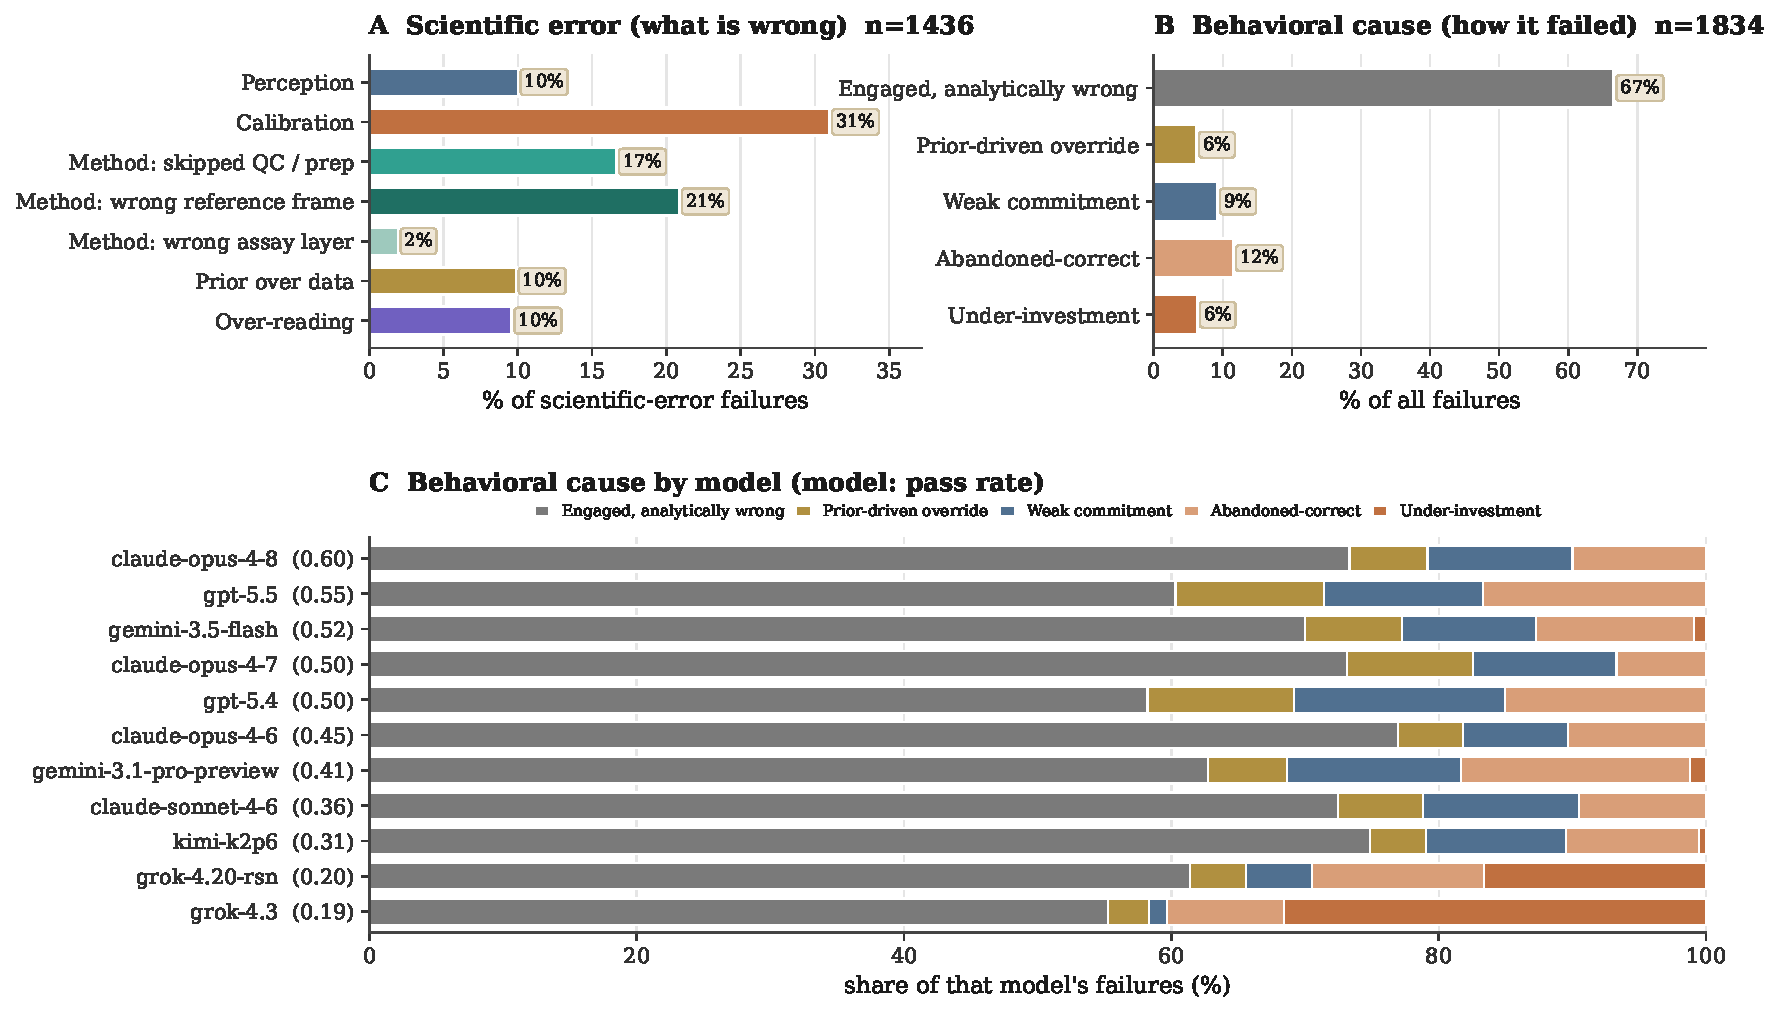
\includegraphics[width=0.91\textwidth]{figures/fig3_failure_taxonomy.pdf}

  \captionof{figure}{\textbf{Expected failure taxonomy.}
  TxBench-PP tasks are designed to distinguish careful preclinical
  pharmacology reasoning from program-relevant judgment gaps: literature priors
  overriding assay evidence, assay-context calibration failures, missing
  multi-property integration, and rigid thresholds. Replace this design
  taxonomy with empirically tagged failure counts after trajectory review.}
  \label{fig:failure-taxonomy}
\end{center}

\StartBody

\subsection{Case examples span the compound-centered preclinical spine}

The benchmark examples should make the task format concrete. In decryptM, a
blinded kinase inhibitor can carry a familiar class label while the
dose-resolved phosphorylation footprint supports a different kinase-family
mechanism. In Kinobeads, the strongest apparent protein signal may be a complex
contaminant rather than a direct binder. In TG-GATEs, a blood-chemistry
threshold may be less informative than pathology and survival under the study
protocol. In PK tasks, total exposure or potency alone can select a compound
that lacks adequate unbound coverage over the dosing interval.

\todo{Replace these examples with exact task names, final answer surfaces, and
short descriptions after the public task manifest is frozen.}

\EndBody

\begin{center}
  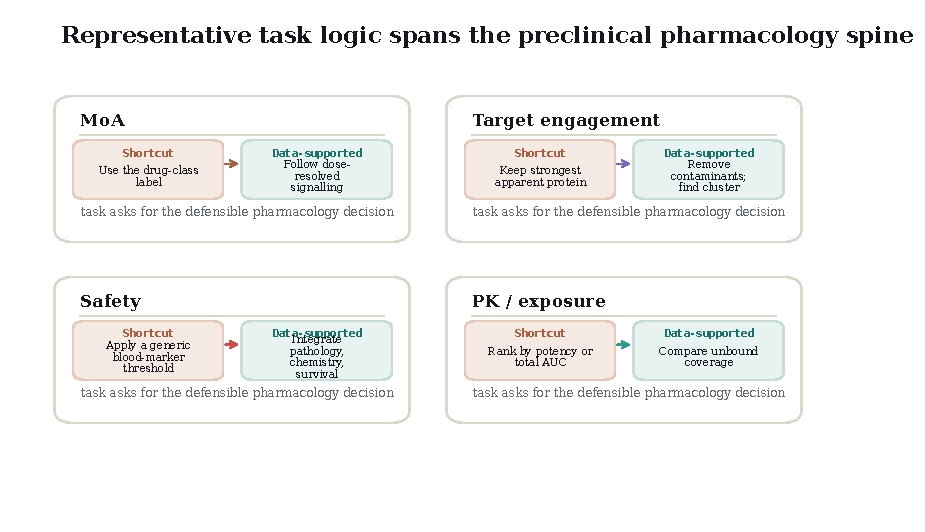
\includegraphics[width=0.92\textwidth]{figures/fig4_cases.pdf}

  \captionof{figure}{\textbf{Representative task logic.}
  Across mechanism, target engagement, safety, and exposure decisions, the
  correct answer is the one supported by the supplied assay evidence, not the
  familiar shortcut.}
  \label{fig:case-examples}
\end{center}

\StartBody

\section{Discussion}

TxBench-PP measures a narrow but important part of drug discovery: whether an
agent can turn preclinical pharmacology evidence into a defensible local
decision. This scope is intentionally smaller than end-to-end therapeutic
discovery. It is a small-molecule cluster benchmark within the broader
TherapeuticsBench roadmap, not a claim to cover every stage or modality. It
does not yet test target genetics, full disease-model selection, primary
screening operations, broad clinical translation, or non-small-molecule
modalities. The narrower scope makes the benchmark verifiable while still
covering decisions that directly affect compound advancement.

The central hypothesis is that current agents will often operate the tools of
preclinical analysis but fail at the scientific judgment layer. If a model
selects a mechanism from a drug label, trusts a contaminated target-engagement
signal, ignores survivor bias, or ranks by total exposure rather than unbound
coverage, it may produce a fluent and computationally elaborate answer that is
not the pharmacology decision supported by the data.

\todo{After results are available, add a paragraph comparing endpoint pass
rates, partial-credit or field-level scores if available, and trajectory
review. Emphasize what capability is missing and which tasks show meaningful
progress.}

Future versions can extend the benchmark upstream to target rationale and
primary screening, sideways to pharmacogenomics and disease-model
characterization, and across modalities to antibodies, ADCs, degraders,
oligonucleotides, cell therapies, and gene therapies. A complementary
long-horizon TherapeuticsBench track can follow program stories across
discovery, development, and translation. For the current paper, the clean claim
should remain: TxBench-PP is a verifiable cluster benchmark for small-molecule
preclinical pharmacology decisions.

\section{Methods}

\subsection{Task construction}

Candidate evaluations are derived from realistic preclinical pharmacology
workflow states. A task is retained when the target conclusion can be recovered
from the supplied files, expressed through a constrained final answer, and
graded deterministically. Tasks should be revised or removed when the prompt
over-specifies the method, when multiple reasonable analyses produce
incompatible decisions, or when the grader cannot distinguish the supported
pharmacology conclusion from a plausible but unsupported answer.

\subsection{Agent runs and aggregation}

\todo{Insert model-harness list, number of attempts per evaluation, execution
environment, parsing rules, and how invalid or missing outputs are counted.}

\subsection{Statistical analysis}

\todo{Insert primary metric and confidence interval convention. If following
SpatialBench/EpiBench, report evaluation-weighted endpoint pass rate, raw pass
counts for interpretability, and Student $t$ confidence intervals over
evaluation-level replicate means.}

\section*{Data availability}

\todo{Insert public repository, public example evaluations, result summaries,
and trajectory availability language.}

{\fontsize{8.3}{10.7}\selectfont
\begin{thebibliography}{99}

\bibitem{zecha2023decryptm} Zecha, J. et al. Decrypting drug actions and
kinase functions by dose-resolved phosphoproteomics. \textit{Science} (2023).

\bibitem{eckert2025decrypte} Eckert, M. A. et al. decryptE: dose-resolved
expression proteomics for compound mechanism analysis. \textit{Manuscript /
dataset reference to verify before submission} (2025).

\bibitem{reinecke2024kinobeads} Reinecke, M. et al. Kinobeads profiling for
chemoproteomic target engagement. \textit{Manuscript / dataset reference to
verify before submission} (2024).

\bibitem{tg-gates} Igarashi, Y. et al. Open TG-GATEs: a large-scale toxicogenomics
database. \textit{Nucleic Acids Research} 43, D921--D927 (2015).

\bibitem{drugmatrix} Ganter, B. et al. DrugMatrix toxicogenomics resource.
\textit{Pharmacogenomics} 6, 715--727 (2005).

\bibitem{prism2020} Corsello, S. M. et al. Discovering the anticancer
potential of non-oncology drugs by systematic viability profiling.
\textit{Nature Cancer} 1, 235--248 (2020).

\bibitem{lincs2017} Subramanian, A. et al. A next generation connectivity map:
L1000 platform and the first 1,000,000 profiles. \textit{Cell} 171,
1437--1452 (2017).

\bibitem{jumpcp2024} Chandrasekaran, S. N. et al. JUMP Cell Painting dataset.
\textit{Manuscript / resource reference to verify before submission} (2024).

\end{thebibliography}
}


\EndBody

\end{document}
